\section{Checking a null}
\label{sec:validate}

A null that changes nothing passes a zero-offset check while reproducing all measured overlap.
This section pairs that necessary check with a positive control that can expose failure to
randomise. We use ``level'' and ``power'' descriptively for null offset and planted-signal
recovery, not for a rejection threshold, test size, or rejection probability.

\subsection{Level is not enough}
\label{sec:level}

The natural check on a null passes a null that does nothing. Build a matched reference pair from
an explicitly specified null generator, pass it through the candidate randomisation, and confirm
that the reported excess has zero offset. Call this the \texttt{H0} check. We report external
finite-draw diagnostics separately from the exact scalar decompositions.

Write $(A_0,B_0)$ for a pair from the constructed reference and let
$\mathcal N_1,\mathcal N_2$ be independent candidate-null draws. The \texttt{H0} statistic is
\begin{equation}
  \mathbb{E}\left[\mathcal{O}(A_0,B_0)-
  \mathcal{O}(\mathcal N_1(A_0),\mathcal N_2(B_0))\right],
  \label{eq:h0}
\end{equation}
and for $\mathcal N=\mathrm{id}$ this is exactly zero. A Haar-orbit self-reference is likewise
idempotent in distribution, so its population \texttt{H0} is exactly zero. The recorded external
\texttt{H0} instead uses independently activation-generated, spectrum-matched endpoints
(Appendix~\ref{app:main}); because that generator is not the conditional orbit law, its offset
mixes reference mismatch, over-destruction, and Monte Carlo error. It is only a stress diagnostic
and is never added to the estimand.
The identity null can therefore earn a perfect score while randomising little of its target.
The asymmetry is not incidental. Eq.~\ref{eq:h0} measures over-destruction, the error that makes
a null report structure where there is none. Under-destruction makes a null report that real
coupling as null-reproduced. The check is blind to that failure mode. It is also relative to the
constructed reference; it neither establishes a unique data-generating null nor supplies a
model-free false-positive rate. The missing diagnostic is a check that can fail under an
alternative.

\begin{figure}[t]
\centering
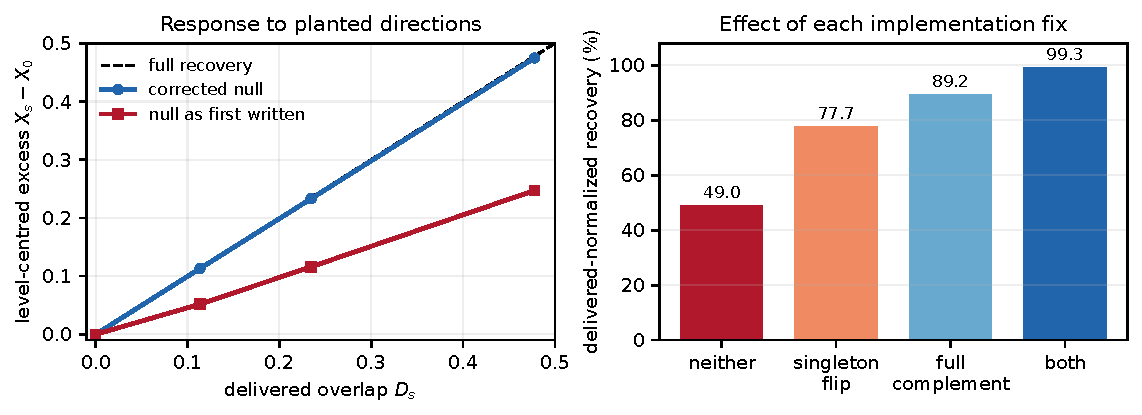
\includegraphics[width=\linewidth]{figures/fig_power.pdf}
\caption{Left: level-centred excess reported against overlap actually delivered by the positive
control. The diagonal is full recovery. Right: level-centred recovery at $s/k=1/4$ with each
activation-null correction enabled separately.}
\label{fig:power}
\end{figure}

\subsection{Power, measured by planting}
\label{sec:power}

The complement of the \texttt{H0} check is a positive control. Take a real task vector $A$ and a
partner $P_0$ drawn from the fitted null, then replace $s$ of the partner's top-$k$ read
directions with directions from $A$, projection/QR-complete the remaining directions, and retain
$P_0$'s singular values to obtain $P_s$ (exact operator in Appendix~\ref{app:power}). The
intervention introduces forced directional matches on top of the pair's pre-existing overlap;
finite-dimensional cross terms mean that it need not add exactly $s/k$.

We therefore normalise by what the intervention actually delivers. For candidate null
$\mathcal N$ define
\begin{align}
 D_s&=\mathbb E[\mathcal O(A,P_s)-\mathcal O(A,P_0)],\nonumber\\
 X_s^{\mathcal N}&=\mathbb E[\mathcal O(A,P_s)-
   \mathcal O(\mathcal N_1(A),\mathcal N_2(P_s))],\qquad
 R_s^{\mathcal N}=\frac{X_s^{\mathcal N}-X_0^{\mathcal N}}{D_s}.
 \label{eq:recovery}
\end{align}
Recovery is thus level-centred and uses delivered rather than nominal overlap. We run this
semi-synthetic stress test on real task vectors and the measured calibration covariance. The
plant preserves singular values but can change the block-occupancy profile on which the null
conditions, so $R_s$ measures sensitivity to this intervention after reconditioning; it is not
power against every possible cross-task dependence or evidence about how the conditioned
statistics arose.

Figure~\ref{fig:power} separates the two arms. The null as first written
recovers only $45.6$--$51.7\%$ of delivered overlap while returning $+0.00004$ at $s=0$, which
looks well behaved under the offset check; the corrected null recovers $99.3$--$99.6\%$ and has
$-0.000623$ at $s=0$. Both arms score the same planted pairs and differ only in the randomisation, which is the
combination we want: small reference offset and high response to the planted alternative. The
study covers four modules and one family of interventions, and planting can alter conditioned
occupancies, so we do not transfer the sub-percent deviation to the $72$-module observational
estimate.

\subsection{What the positive control found}
\label{sec:defects}

The diagnostic exposed two under-randomisation failures in the activation null: its fixed-rank
complement rotation reached only $4$--$18\%$ of that space, and it skipped singleton sign flips
although those directions carry $71\%$ of stored eigenvalue mass. The LoRA generator instead
matched only $\|B\|_F$, letting an uncontrolled factor spectrum set even the sign of its offset.
The zero-offset check missed the first two and had been declared rather than measured for the
third. Appendices~\ref{app:defects} and~\ref{app:ablation} give the fixes and ablation.

\subsection{A common-reference stress test for existing baselines}
\label{sec:baselines}

A reader's first instinct is to substitute some other transform for the isotropic comparator, so we
show how those transforms behave on pairs whose true overlap is zero by construction. We form
semi-synthetic pairs by independently applying our activation-conditioned generator to real
updates. None of the cited work proposes its transform as an evidential null; the rows are
candidate substitutions, not attributed claims. Residual orientation
coupling is absent by construction under this reference, while each endpoint retains its observed
spectrum and occupancy profile. Table~\ref{tab:baselines} reports each baseline's native excess;
these are diagnostics on a common input distribution, not one shared estimand, because whitening
changes the matrices being scored. Because our generator defines the reference, this experiment
neither independently validates our null nor establishes model-free false-positive rates.
\begin{table}[t]
\centering
\caption{Native excess on the same independent-orientation reference pairs, ViT-B/16, $k=8$,
eight fixed modules, and $20$ pairs per module ($160$ total; seed $0$). Exact orthogonality subtracts zero; isotropic subtracts $k/d$;
whitened rows use the participation-ratio floor or all $64$ stored directions before subtracting
$k/d$; the final three rows subtract their
own surrogate mean. Thus entries share overlap units but not an estimand.}
\label{tab:baselines}
\begin{tabular}{@{}lr@{}}
\toprule
baseline & reported excess \\
\midrule
exact orthogonality (no reference subtracted)        & $+0.0275$ \\
isotropic $k/d$                                     & $+0.0171$ \\
whitened at the participation ratio                 & $+0.0522$ \\
whitened, all stored directions                     & $+0.0554$ \\
generative activation model                         & $-0.8959$ \\
coordinate permutation (paired action)              & $-0.0000$ \\
\bottomrule
\end{tabular}
\end{table}

The untransformed reference pair's raw overlap is $0.0275$, or $2.6$ times isotropic chance;
subtracting the isotropic comparator reports $+0.0171$ excess. Whitening changes the scored
matrices and reports still larger native excesses
(Table~\ref{tab:baselines}). A transform introduced
to reduce interference inside a merge therefore need not be calibrated as an evidential baseline.

The mechanism is concentration, and it sharpens with the ridge. $C_H^{-1/2}$ amplifies small
eigendirections and drives both endpoints onto the same few of them: at a Tikhonov ridge of
$\lambda=10^{-4}\bar w$, $96.5\%$ of the whitened read mass lands on the twenty smallest stored
eigendirections, and a chance-overlap pair is reported at $0.7199$. RegMean's published
off-diagonal shrinkage $\alpha=0.9$ returns $0.0931$ on the same pair. Truncating the whitening at
the top $m_{\rm white}$ directions keeps the reference near chance ($0.0394$, $0.0405$, $0.0422$ at
$m_{\rm white}=8,32,64$), which is why we set $m_{\rm white}$ per module from its participation
ratio. The failure is therefore not whitening as such but whitening into directions the
calibration set does not determine.

The coordinate permutation is the useful counterexample. Here the same permutation is applied to
both endpoints, so overlap, and hence its offset, is exactly unchanged; this paired action is a
deliberate counterexample rather than the independent action in Eq.~\ref{eq:h0}. It nevertheless
destroys occupancy relative to fixed $C_H$, so \S\ref{sec:null} rejects it. Passing an offset check
is not sufficient, which is \S\ref{sec:level}'s lesson from the other side.

\subsection{The same test on the LoRA null}
\label{sec:lora-power}

For LoRA, we score only the attainable plant
$P_s^\star=P_sA^+A=(\alpha/r)B_sA$, with $B_s=(r/\alpha)P_sA^+$; both raw and null terms use
$P_s^\star$ (Appendix~\ref{app:lora-power}). It delivers $37.386\%$, $49.790\%$, and $57.043\%$ of the nominal affine increment
at $s=1,2,4$. Normalising the level-centred excess by those delivered increments gives
$101.117\%$, $101.078\%$, and $100.701\%$ recovery. The initial norm-matched generator also has
near-$100\%$ level-centred response, but its unplanted level is $-0.1485$, versus $-0.0073$ after
factor-spectrum matching. The correction therefore calibrates level rather than rescuing low
power or an upward bias. This remains one intervention over four modules and six tasks.

